\newpage

\section{Ricerca}

Un \textbf{albero di ricerca} è dato dall'insieme delle possibili sequenze di
azioni che è possibile applicare a partire da uno stato iniziale.

\textbf{Radice}: contiene lo stato iniziale.

\textbf{Nodi}: contengono gli stati.

\textbf{Rami}: sono le azioni possibili.

Lo stesso stato può comparire più volte in un albero di ricerca $\rightarrow$
possono esserci dei cicli.

\textbf{Nota bene - 1}: il grafo che rappresenta lo spazio degli stati \textbf{è una
cosa diversa dall'albero di ricerca}: l'albero di ricerca può contenere più volte
lo stesso stato.

\textbf{Nota bene - 2}: nodo e stati sono due cose diverse: uno stato è una
configurazione del mondo con cui si ha a che fare e un nodo è una struttura
usata per rappresentare l'albero di ricerca.

\textbf{Foglie}: nodi senza figli.

\textbf{Frontiera}: nodi foglia che si possono espandere.

Il seguente algoritmo \ref{alg:search} riporta come viene svolta la ricerca nell'albero
costruito. 

\begin{algorithm}
    \caption{Algoritmo di ricerca}
    \label{alg:search}
    \begin{algorithmic}[1] % The number tells where the line numbering should start
        \Procedure{TREE SEARCH}{$problem$} \Comment{ritorna una soluzione o fallisce}
			\State Inizializza la frontiera usando lo stato iniziale del problema
            \Loop
            \If{Frontiera vuota} \Return{Fallimento} \EndIf
            \State Scegli un nodo foglia e rimuovilo dalla frontiera
            \If{Nodo con stato obiettivo} \Return{Soluzione} \EndIf
            \State Espandi il nodo scelto e aggiungi il risultato alla frontiera
			\EndLoop
        \EndProcedure
    \end{algorithmic}
\end{algorithm}

Questo algoritmo può produrre dei cicli. Una soluzione possibile è la seguente,
che considera un insieme \textbf{explored set} che memorizza ogni nodo espanso.

\begin{algorithm}
    \caption{Algoritmo di ricerca senza cicli}
    \label{alg:search2}
    \begin{algorithmic}[1] % The number tells where the line numbering should start
        \Procedure{TREE SEARCH}{$problem$} \Comment{ritorna una soluzione o fallisce}
			\State Inizializza la frontiera usando lo stato iniziale del problema
			\State Inizializza l'insieme explored set (vuoto all'inizio).
            \Loop
            \If{Frontiera vuota} \Return{Fallimento} \EndIf
            \State Scegli un nodo foglia e rimuovilo dalla frontiera
            \If{Nodo con stato obiettivo} \Return{Soluzione} \EndIf
			\State Aggiungi il nodo all'insieme explored set
            \State Espandi il nodo scelto e aggiungi il risultato alla
frontiera \textbf{solo se} non è già nella frontiera e nemmeno nell'explored
set 
			\EndLoop
        \EndProcedure
    \end{algorithmic}
\end{algorithm}

\subsection{Proprietà}

La frontiera deve essere una struttura dati che memorizzi i nodi in modo tale
che si possa scegliere facilmente il prossimo nodo da espandere.

La struttura dati appropriata per questo è una \textbf{coda}.

Esistono diverse politiche di ordinamento di una coda \dots

\begin{itemize}
\item FIFO: l'operazione pop ritorna l'elemento più vecchio inserito.
\item LIFO: l'operazione pop ritorna l'elemento più recente inserito (in questo
caso si chiama ``stack'')
\item Coda di priorità: l'operazione pop ritorna l'elemento con priorità più alta.
\end{itemize}

Una \textbf{strategia di ricerca} è definita in base all'ordine di espansione
dei nodi nell'albero e viene valutata in base ai seguenti parametri:

\begin{itemize}
\item \textbf{Completezza} - Trova sempre una soluzione, se questa esiste?
\item \textbf{Complessità di tempo} - Quanto tempo impiega? (di solito si
esprime come una funzione dei dati di input)
\item \textbf{Complessità di spazio} - Di quanta memoria ha bisogno?
(di solito si esprime come una funzione dei dati di input)
\item \textbf{Ottimalità} - È in grado di trovare una soluzione ottima,
se questa esiste?
\end{itemize}

Le complessità di tempo e spazio si misurano in base a:

\begin{itemize}
\item \textbf{b} - Il massimo \textbf{fattore di branching} nell'albero di
ricerca
\item \textbf{d} - Profondità del minore nodo con uno stato obiettivo
\item \textbf{m} - La lunghezza massima di ogni cammino nello spazio degli
stati
\end{itemize}

Il tempo si misura in termini di \textbf{nodi totali generati durante la
ricerca}.

Lo spazio si misura in termini del \textbf{massimo numero di nodi
memorizzati}.\\

\subsection{Tipi di ricerca}

\textbf{Breadth-first search}: espande il nodo minore non ancora esplorato.
La frontiera è una coda FIFO.

È completo (se b è finito), ha complessità di spazio e tempo pari a
$\mathcal{O}(b^d)$, è ottimale (se ha un costo di un'unità per passo).
Lo spazio qui è il problema maggiore.\\

\begin{figure}[H]
\centering
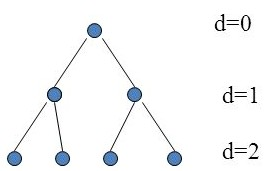
\includegraphics[width=0.35\textwidth]{breadth.jpg}
\caption{A ogni livello i, la complessità è $b(d^i)$}
\label{fig:breadth}
\end{figure}

\textbf{Uniform-cost search}: espande il nodo non ancora esplorato con minor costo.
La frontiera è una coda di priorità in base al costo di cammino.
È equivalente al breadth-first se i costi sono tutti uguali.

Se i costi per ogni azione sono maggiori di una costante $\epsilon$, allora ha
complessità di spazio e tempo pari a $\mathcal{O}(b^{floor(C^*/\epsilon)+1})$
dove $C^*$ è il costo della soluzione ottimale.
\textbf{È ottimale ed è completo}.

È diverso dall'euristica best first search perché considera la lunghezza di
tutti i cammini correnti e non solo il costo dell'azione corrente.\\

\textbf{Depth-first search}: espande il nodo non ancora esplorato più profondo
(più lontano dalla radice) dell'albero. La frontiera è uno stack (politica LIFO).
\textbf{Non} è completo in generale dato che uno stato già incontrato non può
essere ripetuto in un cammino. In spazi finiti è completo. Non è ottimale.
Complessità di spazio pari a: $\mathcal{O}(bm)$ (lineare).
Complessità di tempo pari a: $\mathcal{O}(b^m)$\\

\textbf{Depth-limited search}: la ricerca si ferma alla profondità p.
Ricordando che d è la profondità del minor nodo con uno stato obiettivo,
questo algoritmo non è completo se p < d (non fa in tempo a raggiungere una
soluzione) e non è ottimale se p > d (cerca più di quanto necessario, può
trovare soluzioni con costo maggiore).\\

\textbf{Iterative deepening search}: applica la depth-limited search incrementando
p a ogni iterazione.

\begin{algorithm}
    \caption{Iterative deepening search}
    \label{alg:search2}
    \begin{algorithmic}[1] % The number tells where the line numbering should start
        \Procedure{ITERATIVE-DEEPENING-SEARCH}{$problem$} \Comment{ritorna una
soluzione o fallisce}
            \For{depth=0 to $\infty$}
            \State Risultato $\leftarrow$ DEPTH-LIMITED-SEARCH(problem, depth)
            \If{Risultato $\neq$ fallimento} \Return{Risultato} \EndIf
			\EndFor
        \EndProcedure
    \end{algorithmic}
\end{algorithm}

È completo.
È ottimale se il costo del cammino è una funzione \textbf{crescente con
la profondità}.
Complessita di spazio pari a: $\mathcal{O}(bd)$ (lineare).
Complessità di tempo pari a: $\mathcal{O}(b^d)$\\
